%!TEX root = ../../Main.tex
\graphicspath{{Chapters/Display/}}
%-------------------------------------------------------------------------------


\section{Display driver}
Igennem øvelser til undervisningen, er der blevet opbygget en driver til et grafisk display. Igennem processen til dette projekt er der blevet modificeret og arbejdet videre på selvsamme driver. Cpp filen ligger under TFTdriver, som er bygget op af flere forskellige funktioner. I dette afsnit vil der gives et overblik over de mest essentielle funktioner. For at få en forståelse af selve opbygningen af driveren, henvises til datasheet for controlleren. 
\href{https://blackboard.au.dk/bbcswebdav/pid-1697983-dt-content-rid-3847230_1/courses/BB-Cou-UUVA-73302/BB-Cou-UUVA-65758_ImportedContent_20170106021228/BB-Cou-STADS-UUVA-52360_ImportedContent_20160107025559/LAB/Lab3a%20Graphic%20LCD%20Display/Files%20for%20LAB3a/ILI9341_v1.11.pdf}{ILI9341} \\
For at opbygge en basisforståelse for driveren, vil der først blive forklaret DisplayInit(). Først sætter vi de porte vi skal bruge fra Arduino til hhv. indgange og udgange. Vi har dog valgt ikke at have tilbagemeldinger, og derfor er der ikke initialiseret nogle indgange. Herefter sætter vi RESET, CS, WRX, RDX høje ift figur \ref{fig:Bus_timing}. Der bliver kørt en reset (tjek lige koden med timing, burde være kortere), for at resette displayet, og bagefter sendt fire kommandoer, som kan findes i command list i databladet. Sleep Out, Display On, Pixel format set = 16 bit og Memory Access Control (BGR = 1) (Tjek ift henning hvad dette gør). 



\begin{figure}[H]
	\centering
	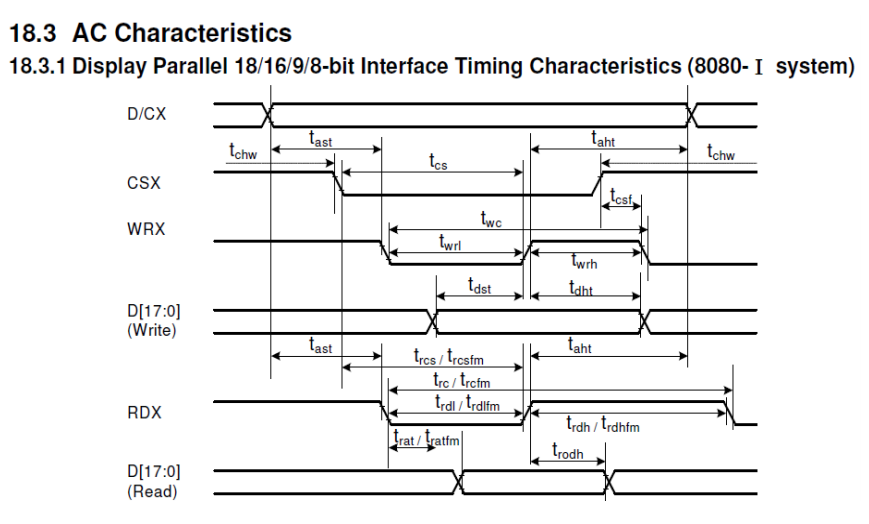
\includegraphics[width = 400 pt]{Img/Bus_timing.png}
	\caption{Bus Timing}
	\label{fig:Bus_timing}
\end{figure}

Herunder vil de essentielle funktioner deles op i hvert sin tabel. Flere af funktionerne gør brug af både Writecommand() og Writedata(), som er opbygget udfra Bus Timing figur \ref{fig:Bus_timing}. Derudover bruger flere af funktionerne SetColumnAddress() og SetPageAddress(), som er bygget op fra datasheet 8.2.20. og 8.2.21.: \\

\newpage
\textbf{\Large Included Font:}

\begin{center}
\begin{tabular}{ |l|l|l| }
\hline
\multicolumn{1}{ |c| }{\textbf{character.h}} \\
\hline
Karakter størrelse: 24*24 pixels  \\
Antal karakter: 95\\
\hline

\end{tabular}
\end{center} 
\begin{figure}[H]
	\centering
	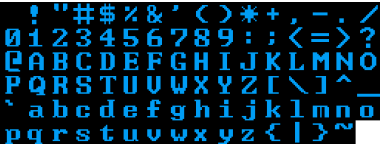
\includegraphics[width = 150 pt]{Img/Thedotfactory.png}
	\caption{The Dot Factory karakter}
	\label{fig:Thedotfactory}
\end{figure}

\textbf{\Large Funktions:}

\begin{center}
\begin{tabular}{ |l|l|l| }
\hline
\multicolumn{1}{ |c| }{\textbf{ FillRectangle(StartX,StartY, Width, Height, Red, Green, Blue)}} \\
\hline
Funktion som laver en firkant med den valgte baggrundsfarve  \\
\hline
\textbf{Paramentre:}  \\ StartX: Startværdi på x-aksen \\StartY: Startværdi på y-aksen\\ Width: Bredden på firkanten\\ Height: Højde på firkanten\\ Red: farve(værdi)\\ Green: farve(værdi) \\ Blue: farve(værdi)\\
\hline
\end{tabular}
\end{center} 

FillRectangle er en funktion som visuelt kan ændre bits til en anden farve på den givne skærm. Fra input vælges startx og starty samt længde og bredde. Derefter laves en ud fra de input der er givet. Farven afhænger også af inputtet. Det der reelt sker, er at den givne farve bliver skrevet til hver eneste pixel, i det sted der er valgt en firkant. 

\begin{center}
\begin{tabular}{ |l|l|l| }
\hline
\multicolumn{1}{ |c| }{\textbf{ drawletters(str[],startx, starty,Red, Green, Blue)}} \\
\hline
Funktion som modtager en en streng, og konverterer ascii værdien til \\den rette værdi ift character.h \\
\hline
\textbf{Paramentre:}  \\str[]: Modtager en streng\\  Startx: Startværdi på x-aksen \\Starty: Startværdi på y-aksen\\ Red: farve(værdi)\\ Green: farve(værdi) \\ Blue: farve(værdi)\\
\\

\hline
\end{tabular}
\end{center}  

drawletters er en startfunktion til drawXletter, i denne funktion, findes længden på den på det givne tegn, som skal skrives. Herudover findes lægden at det givne loop drawXletter skal fortsætte, ift hvor mange bytes der hører til det givne tegn. Denne funktion står for at finde de respektive værdier fra array\_carrier, og sende dem med til drawXletter.  til sidst sættes den nye start\_x, hvor næste tegn kan placeres, her er der valgt et mellemrum fra udvikleren på 1 pixel.

\begin{center}
\begin{tabular}{ |l|l|l| }
\hline
\multicolumn{1}{ |c| }{\textbf{ drawXletter( bitmap[],length,count,startx,starty, letter, modulus,Red, Green, Blue)}} \\
\hline
Funktion som står for at skrive til hver bit, med værdier fra letterhelper()\\
\hline
\textbf{Paramentre:}  \\bitmap[]: Henter en byte fra character.h\\ length: Fortæller funktionen, hvor bred karakteren der skal skrives er\\ count: hvor mange bytes funktionen skal køre igennem for at lave hele karakteren\\ Startx: Startværdi på x-aksen \\Starty: Startværdi på y-aksen\\ Red: farve(værdi)\\ Green: farve(værdi) \\ Blue: farve(værdi)\\
\textbf{Note:} Funktionen sletter gamle karakterer, da en ny smallere karakter end forrige stadig\\ vil forblive på displayet\\

\hline
\end{tabular}
\end{center}  

drawXletters står for at farve hver pixel, så der laves det tegn som er anmodet, dette sker ved at funktionen modtager information fra drawletters, som har information om tegn[], som er hentet fra character.h. Dette array, består af et bitmap af alle ascii tegn, og byte værdier som tegner hver pixel. Igennem funktionen sikres at bredden på tegnet overholdes, og et nyt startx punkt bliver sat, samtidig med at starty (colum) sættes til næste linje. dette gøres indtil den del af arrayet er løbet igennem som er givet fra drawletters. Til sidst i koden slettes (pixels = hvid) tegn eller pixels, som ligger forand det nye tegn som er tegnet. Dette sker for at sikre at tegnene ikke flyder ind over hinanden, hvis der findes gamle tegn på pladsen, hvor den nye tegnes. 



